\begin{frame}[fragile]{\texttt{data/}}
    \begin{columns}
        \begin{column}{0.33\textwidth}
            \begin{figure}
                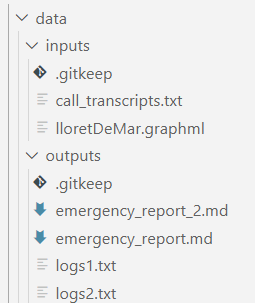
\includegraphics[width=\textwidth]{figures/data_folder_structure.png}
            \end{figure}
        \end{column}
        \begin{column}{0.67\textwidth}
        
    
            \begin{lstlisting}[language=Python]
@start()
def get_call_transcript(self):
    with open(EMERGENCY_CALL_TRANSCRIPTS_FILENAME, "r") as f:
        self.state.call_transcript = f.readlines()[TRANSCRIPT_INDEX]
            \end{lstlisting}
            \begin{lstlisting}[language=Python]
@listen("save full emergency report")
def save_full_emergency_report(self):
    full_emergency_report = f"""
# Emergency Report

## Call Transcript
{self.state.call_transcript}
...
"""
with open(EMERGENCY_REPORT_FILENAME, "w") as f:
    f.write(full_emergency_report)
            \end{lstlisting}
        \end{column}
    \end{columns}
\end{frame}